\label{chap:developpement_embarque}

Une fois le circuit électrique validé par les différents essais réalisés sur breadboard et le \acrshort{pcb} commandé, le développement du logiciel embarqué de l'ESP-32 peut débuter. Ce chapitre présente la conception du programme développé en langage C++ ainsi que les différents outils et bibliothèques utilisés.

Le logiciel embarqué a pour objectif d'assurer la gestion complète du système. Il réalise notamment l'acquisition des données provenant des capteurs, le traitement de ces informations selon l'algorithme de contrôle défini (\acrshort{pid}), ainsi que la commande des différents actionneurs. Il assure également la communication avec l'interface utilisateur.

Le développement est réalisé en plusieurs étapes. Dans un premier temps, l'environnement de développement ainsi que les bibliothèques utilisées sont présentés. Ensuite, l'architecture générale du programme est détaillée afin d'expliquer l'organisation du code et le déroulement de son exécution. Enfin, les différentes fonctions permettant le pilotage des périphériques matériels sont décrites.

L'intégralité du code source est disponible à l'annexe \ref{annexe:code_source_embarque}.

\section{Méthode et outils}


\subsection{Visual Studio Code et PlatformIO}

Le développement du logiciel embarqué est réalisé avec l'environnement Visual Studio Code associé à l'extension PlatformIO. Ce choix permet de bénéficier d'un environnement complet dédié aux systèmes embarqués, regroupant la gestion du projet, la compilation, le téléversement du programme ainsi que la gestion des bibliothèques.

PlatformIO agit comme un intermédiaire entre le code source écrit en C++ et le microcontrôleur ESP-32. Lors de la compilation, le code est transformé en un firmware exécutable par l'ESP-32. Celui-ci est ensuite automatiquement transféré dans la mémoire Flash du microcontrôleur via l'interface USB.

L'utilisation de PlatformIO permet également de définir précisément la configuration matérielle utilisée au travers du fichier \texttt{platformio.ini}. Celui-ci contient notamment le modèle de carte, le framework utilisé ainsi que les différentes dépendances nécessaires au projet.


\subsection{Bibliothèques Arduino}

Le programme est développé en utilisant le framework Arduino intégré à PlatformIO. Celui-ci fournit une couche d'abstraction permettant de simplifier l'utilisation des périphériques internes de l'ESP-32, notamment la gestion des entrées/sorties numériques, des communications série ou encore des interruptions.

Différentes bibliothèques sont utilisées afin de faciliter l'interaction avec les composants externes. Ces bibliothèques permettent notamment de communiquer avec les drivers moteurs via UART, de récupérer les données provenant de l'\acrshort{imu} via le protocole I2C, ainsi que de gérer les différentes communications nécessaires au fonctionnement du système.

L'utilisation de bibliothèques existantes permet de réduire la complexité du développement tout en conservant un contrôle suffisant sur les paramètres de bas niveau nécessaires au fonctionnement du système.


\section{Architecture}

\begin{figure}[H]
    \centering
    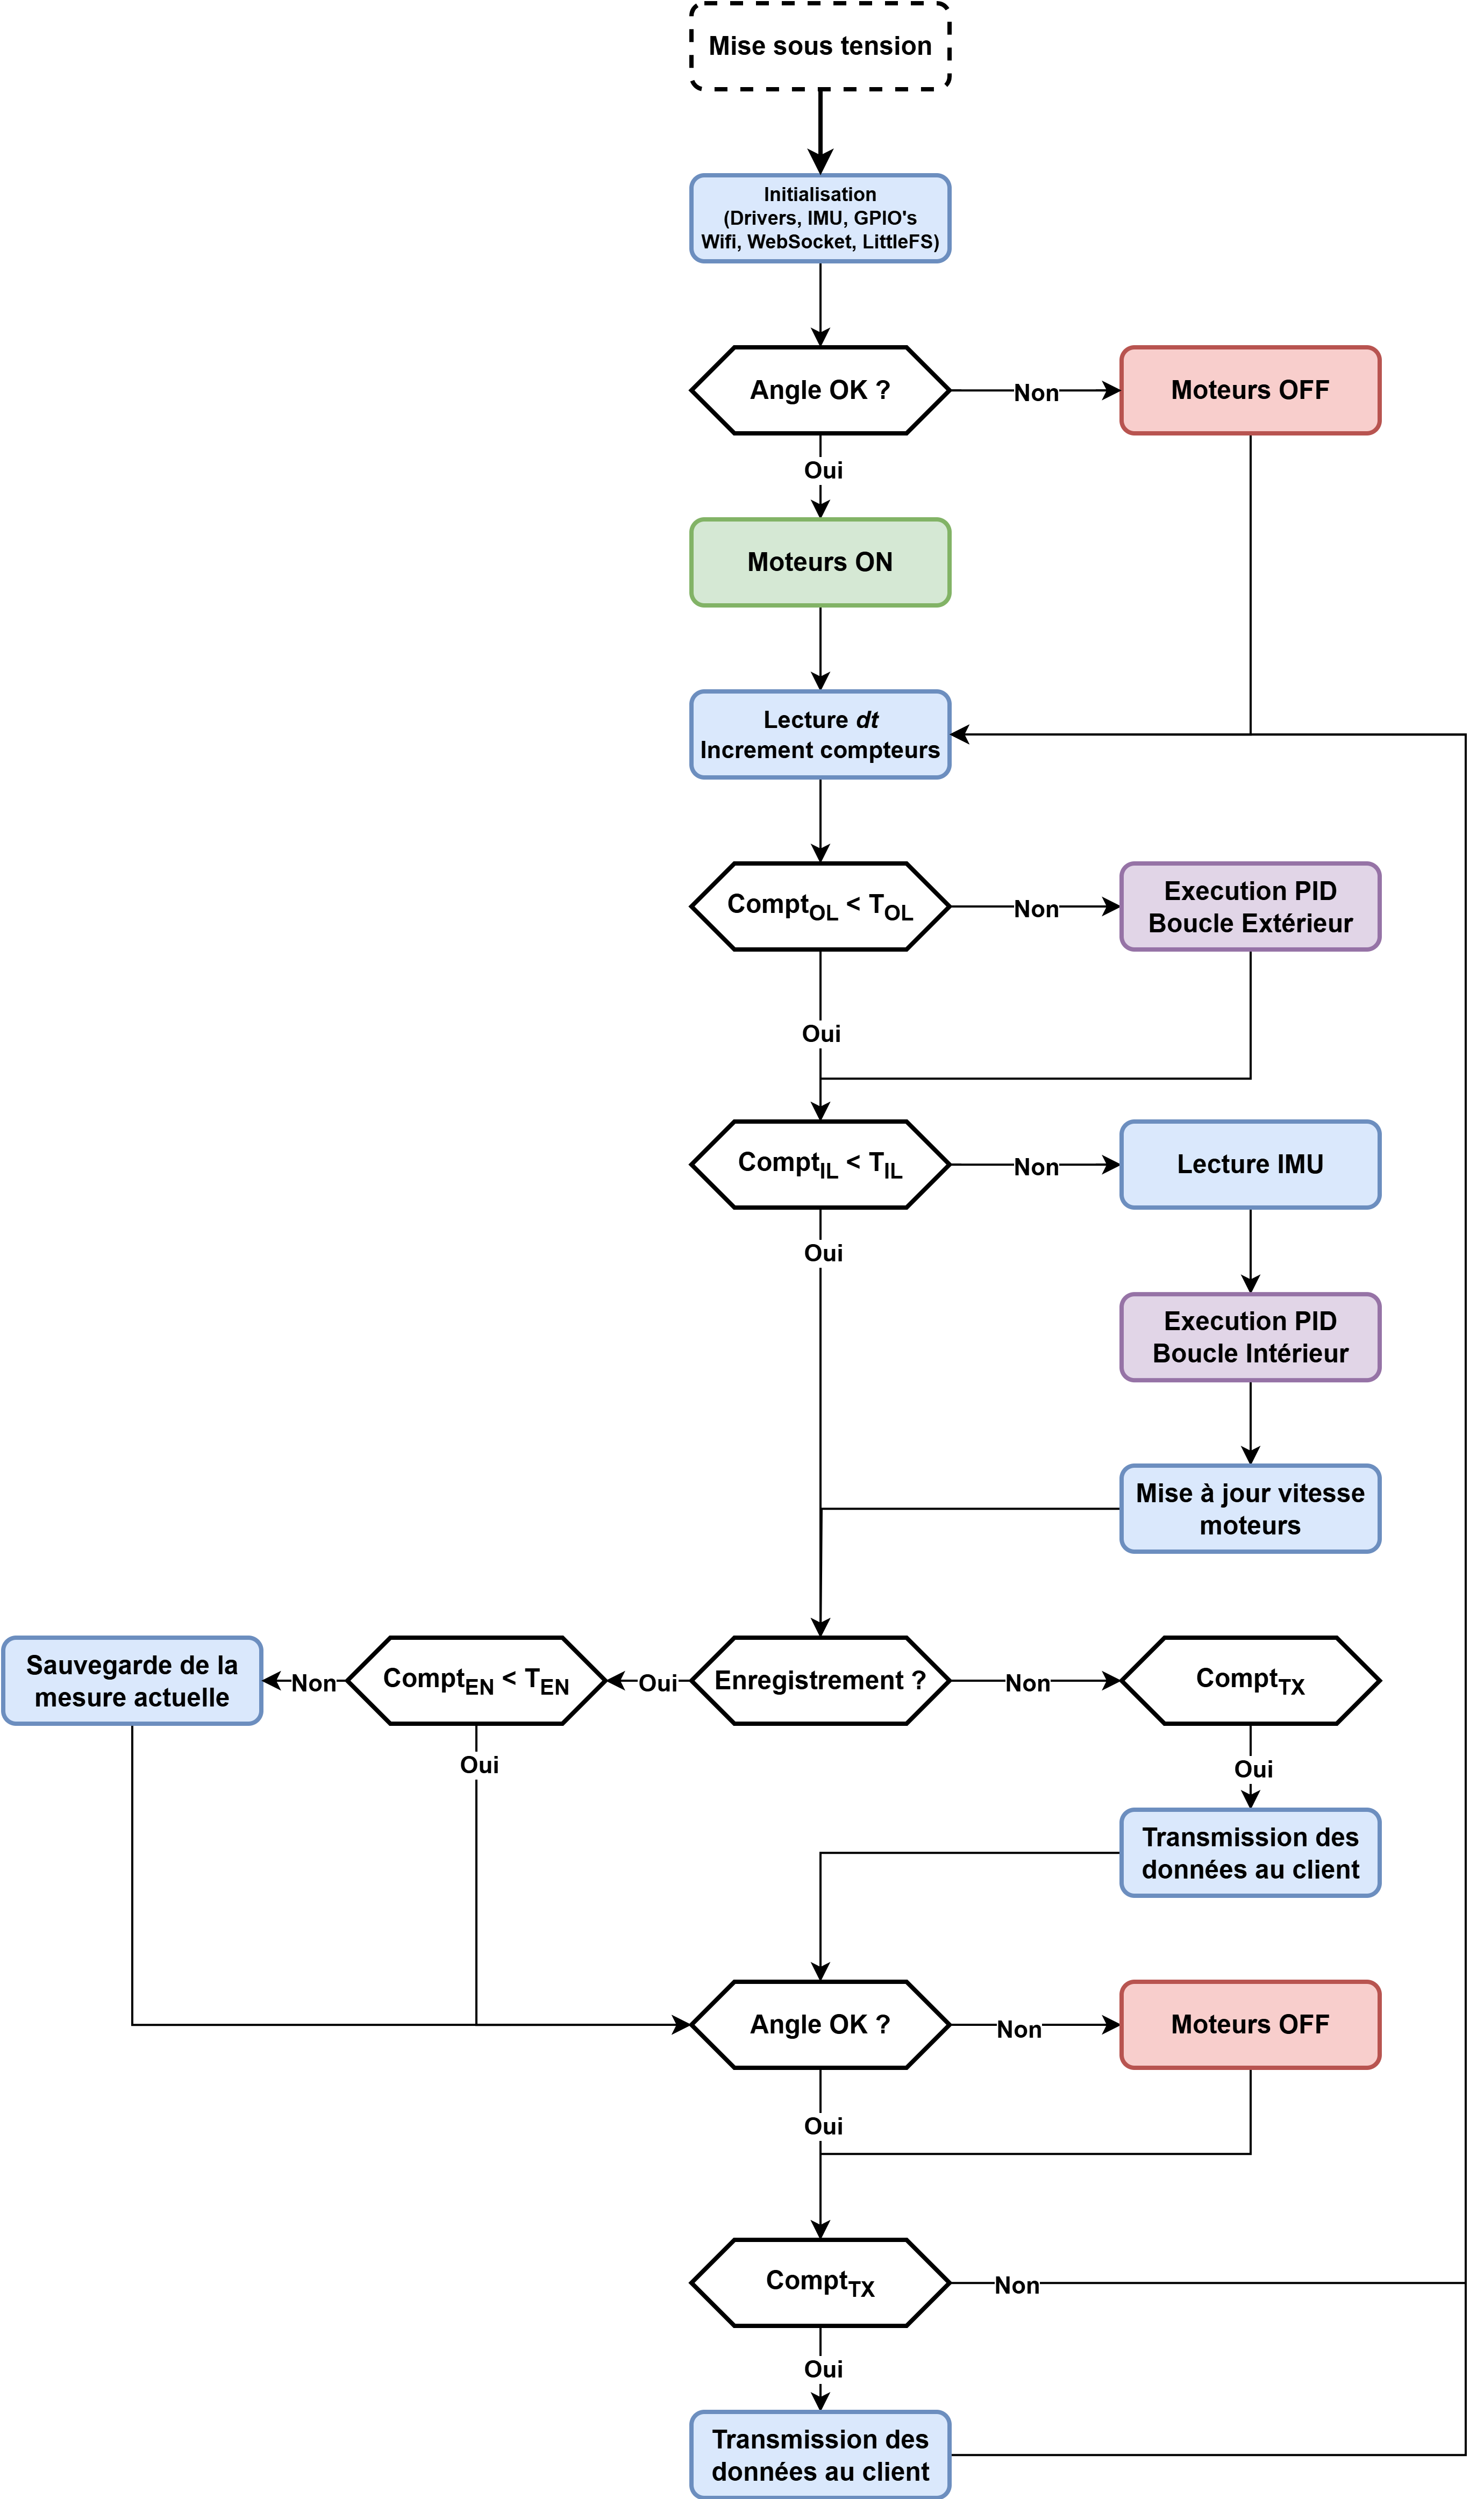
\includegraphics[width=0.8\textwidth]{assets/schemas/schema_bloc_algo_embarque.png}
    \caption{Machine d'état du système embarqué}
    \label{fig:machine d'etat embarque}
\end{figure}
Le programme développé est organisé autour d'une architecture cyclique classique des systèmes embarqués. Après une phase d'initialisation permettant de configurer les différents composants matériels et logiciels, le microcontrôleur exécute continuellement une boucle principale chargée d'assurer le fonctionnement du système.

La séparation entre l'initialisation et l'exécution permet de structurer le programme et de faciliter sa maintenance. Les différentes fonctionnalités sont regroupées en modules indépendants afin de limiter les interactions entre les parties du code.


\subsection{Initialisation}

Au démarrage de l'ESP-32, lors de la mise sous tension du système, une phase d'initialisation est exécutée une unique fois. Cette étape a pour objectif de configurer l'ensemble des ressources matérielles et logicielles nécessaires au fonctionnement du programme.

Les différentes initialisations sont réalisées de manière séquentielle dans l'ordre suivant :

\begin{itemize}
    \item Initialisation de l'interface série UART1, utilisée pour la communication de débogage avec un ordinateur ;
    \item Initialisation des drivers moteurs TMC2226. Cette étape comprend notamment la configuration des registres internes nécessaires au fonctionnement des moteurs (voir \ref{subsection:drivers_moteurs}) ;
    \item Initialisation du module \acrshort{imu} MPU6050 via le protocole I2C;
    \item Configuration du convertisseur analogique-numérique (ADC) utilisé pour mesurer la tension issue du pont diviseur et ainsi estimer le niveau de charge de la batterie ;
    \item Démarrage de la connexion WiFi permettant les communications avec l'interface utilisateur ;
    \item Initialisation du système de fichiers LittleFS utilisé pour le stockage des ressources nécessaires au serveur web ;
    \item Initialisation du serveur WebSocket permettant une communication bidirectionnelle avec l'interface utilisateur ;
    \item Démarrage du serveur web chargé de fournir les différentes ressources accessibles depuis un navigateur ;
    \item Attente de $50~ms$ afin de laisser le temps aux différents périphériques de terminer leur démarrage.
    \item Activation ou Désactivation des moteurs en fonction de la gamme d'angle autorisée.
\end{itemize}

Cette phase garantit que l'ensemble des composants du système est correctement configuré avant le début de l'exécution cyclique du programme. Une fois cette séquence terminée, l'ESP-32 entre dans sa boucle principale, durant laquelle les acquisitions, les calculs de contrôle et les commandes des actionneurs sont exécutés continuellement.

\subsection{Boucle principale}

Après l'initialisation, l'ESP-32 exécute continuellement la boucle principale du programme. Cette boucle constitue le cycle d'exécution du système et regroupe l'ensemble des opérations nécessaires au contrôle du robot.

Afin de respecter les contraintes temporelles du système de contrôle, certaines opérations ne sont pas exécutées à chaque itération de la boucle principale, mais uniquement lorsque leur période d'exécution respective est atteinte. Cette méthode permet de séparer les différentes tâches selon leur fréquence d'exécution et d'optimiser l'utilisation des ressources du microcontrôleur.

À chaque itération de la boucle principale, les opérations suivantes sont réalisées dans l'ordre :

\begin{itemize}
    \item Lecture du temps écoulé depuis la dernière exécution des différentes tâches périodiques ;
    
    \item Si le temps écoulé dépasse la période d'exécution de la boucle externe $T_{OL}$ (\textit{Outer Loop}), l'algorithme \acrshort{pid} associé à cette boucle est exécuté. Cette boucle permet notamment de déterminer la consigne nécessaire au maintien de la position souhaitée du système ;
    
    \item Si le temps écoulé dépasse la période d'exécution de la boucle interne $T_{IL}$ (\textit{Inner Loop}), la mesure de l'angle est acquise depuis le capteur \acrshort{imu}. L'algorithme \acrshort{pid} de la boucle interne est ensuite exécuté afin de calculer la consigne de vitesse appliquée aux moteurs ;
    
    \item Si le mode d'enregistrement est activé, les différentes données du système sont sauvegardées. Cette acquisition est réalisée dans la boucle interne afin de conserver une résolution temporelle suffisante pour l'analyse du comportement du système ;
    
    \item Si l'angle mesuré par l'\acrshort{imu} dépasse les limites de fonctionnement définies, une sécurité est déclenchée et les moteurs sont désactivés afin d'éviter une perte de contrôle ou un endommagement du système.

    \item Si le temps écoulé dépasse la période de transmission des données mesuré $T_{TX}$, le serveur (ESP32) transmet au client des informations relatives aux différentes grandeurs (\texttt{batterie,angle,target\_angle}), il faut noter qu'il existe en réalité un compteur pour chacun des éléments à transmettre.

\end{itemize}

Cette organisation permet d'obtenir une architecture de contrôle à plusieurs fréquences d'exécution. La boucle interne, exécutée plus rapidement, assure la stabilisation dynamique du système, tandis que la boucle externe, exécutée à une fréquence plus faible, permet de gérer les consignes globales du robot.
\subsection{Interruptions}

La boucle principale assure la stabilisation et le maintien de l'équilibre du robot. Cependant, afin de permettre à l'utilisateur d'interagir avec le système et de modifier son comportement en temps réel, des événements externes doivent également pouvoir être pris en compte.

Ces événements sont générés par l'interface de contrôle utilisateur (présentée dans la section correspondante). Les commandes envoyées par l'utilisateur sont transmises à l'ESP-32 via une communication WebSocket. Les données reçues contiennent notamment les informations nécessaires au pilotage du robot, telles que les consignes de déplacement ou les paramètres de fonctionnement.

Lorsqu'une nouvelle donnée est reçue via WebSocket, une fonction de rappel (\textit{callback}) est exécutée afin de traiter l'information reçue. Cette fonction ne réalise pas directement les actions de contrôle, mais met à jour des variables globales accessibles depuis la boucle principale.

\subsubsection{Commandes WebSocket}
\label{subsubsection:web_socket}
Les commandes WebSocket permettent au client d'envoyer des instructions au serveur embarqué. Chaque commande est identifiée par un identifiant (\texttt{msg\_id}) correspondant à une action spécifique.
Les messages échangés via WebSocket peuvent être initiés par le client ou par le serveur. La colonne \textit{Direction} indique le sens de communication associé à chaque identifiant de message.
Ici, le client représente l'utilisateur et le serveur représente l'ESP-32.

\begin{table}[H]
\centering
\begin{tabularx}{\textwidth}{|l|l|X|}
\hline
\multicolumn{3}{|c|}{\textbf{Client $\rightarrow$ Serveur}} \\
\hline
\textbf{msg\_id} & \textbf{msg} & \textbf{Description} \\
\hline
\texttt{motors\_off} & "" & Désactivation des moteurs. \\
\hline
\texttt{motors\_on} & "" & Activation des moteurs si les conditions de sécurité sont respectées. \\
\hline
\texttt{calibrate} & "" & Sauvegarde de l'angle actuel comme référence d'équilibre. \\
\hline
\texttt{pid\_values} & PID & Mise à jour des paramètres des correcteurs PID. \\
\hline
\texttt{pid\_request} & "" & Demande des paramètres PID actuels. \\
\hline
\texttt{joystick-left} & \texttt{"y"} & Modification de la consigne de vitesse. \\
\hline
\texttt{joystick-right} & \texttt{"x"} & Modification de la consigne de rotation. \\
\hline
\end{tabularx}
\caption{Commandes WebSocket reçues par le serveur}
\end{table}

\begin{table}[H]
\centering
\begin{tabularx}{\textwidth}{|l|l|X|}
\hline
\multicolumn{3}{|c|}{\textbf{Serveur $\rightarrow$ Client}} \\
\hline
\textbf{msg\_id} & \textbf{msg} & \textbf{Description} \\
\hline
\texttt{motor\_state} & \texttt{"value"} & Indique l'état actuel des moteurs. \\
\hline
\texttt{calibration\_angle} & \texttt{"value"} & Retourne l'angle de calibration enregistré. \\
\hline
\texttt{pid\_values} & PID & Retourne les paramètres PID actuellement utilisés. \\
\hline
\texttt{battery} & "votage","percentage" & Transmets les données de la batterie \\
\hline
\texttt{target\_angle} & "value" & Transmets la valeur de \texttt{target\_angle} \\
\hline
\texttt{angle} & "value" & Transmets la valeur de l'angle actuel \\
\hline
\end{tabularx}
\caption{Informations WebSocket envoyées par le serveur}
\end{table}

Cette séparation permet de conserver une architecture claire : la réception des commandes est gérée de manière asynchrone, tandis que leur application effective reste effectuée dans la boucle principale. Celle-ci conserve ainsi la maîtrise du déroulement temporel de l'algorithme de contrôle.

Ainsi, les commandes utilisateur peuvent modifier le comportement du robot sans perturber l'exécution des boucles de contrôle temps réel nécessaires au maintien de l'équilibre.

Les commandes suivantes: \texttt{battery, target\_angle, angle} sont transmises par le serveur périodiquement. La période d'envoi est réglée par des defines.
\section{Pilotage des périphériques}
Une fois le fonctionnement principal du code embarqué décrit, il est possible d'aller dans les détails concernant la manière dont les différents périphériques sont pilotés. 

\subsection{Drivers moteurs}
\label{subsection:drivers_moteurs}
Les drivers moteurs, TMC2226 \cite{TMC2226_datasheet} peuvent êtres interfaçés via UART bi-directionnel, comme indiqué plus haut. Une bibliothèque a donc été réalisée de 0 afin de pouvoir communiquer avec les différents registres.

La bibliothèque inclue la création d'une classe TMC2226, la gestion de l'UART bi-directionnel.
\subsubsection{Initialisation des drivers}

Avant de pouvoir piloter les moteurs, chaque driver TMC2226 doit être correctement initialisé. Cette étape consiste tout d'abord à configurer l'interface UART de l'ESP32 avec les paramètres imposés par le datasheet UART 500000 Baud 8N1.

Une fois la liaison série opérationnelle, plusieurs registres de configuration du TMC2226 sont initialisés. Le registre \texttt{GCONF} est configuré afin de désactiver le mode \texttt{PDN} (\texttt{pdn\_disable = 1}), permettant ainsi d'utiliser l'interface UART comme moyen principal de communication. Le bit \texttt{mstep\_reg\_select} est également activé afin que la résolution de micro-pas soit définie par le registre \texttt{CHOPCONF} plutôt que par les broches matérielles. Les options \texttt{scale\_analog} et \texttt{multistep\_filt} sont également activées afin d'utiliser la référence analogique du courant moteur $V_{ref}$ et d'améliorer la fluidité du mouvement grâce au filtrage des micro-pas.
Le courant est donc séléctionné par le potentiomètre et pas le registre correspondant.

Enfin, chaque driver est identifié par une adresse UART. Le protocole de communication du TMC2226 permet de distinguer plusieurs circuits connectés sur un même bus grâce à une adresse codée sur deux bits. Cette adresse est définie matériellement à l'aide des broches \texttt{MS1} et \texttt{MS2}, qui servent à la fois à sélectionner la résolution des micro-pas au démarrage et l'adresse UART du composant. Dans le cadre de ce projet, deux adresses différentes ont été utilisées (\texttt{0b00} et \texttt{0b01}) afin de pouvoir communiquer indépendamment avec plusieurs drivers partageant la même ligne UART. La bibliothèque développée prend en charge cette adresse lors de la construction de chaque instance de la classe \texttt{TMC2226}, permettant ainsi d'envoyer les commandes au driver concerné sans conflit avec les autres périphériques présents sur le bus.

\subsubsection{Contrôle vitesse}
Lors du test avec le breadboard, les pins STP et DIR étaient alors utilisées afin de contrôler ces derniers. Cependant, en parcourant le datasheet du TMC2226, il existe un registre permettant
de faire fonctionner les moteurs à vitesse constante sans impulsions requises. Il s'agit du registre \texttt{V\_actual}. (P.28 du Datasheet)
\begin{figure}[H]
    \centering
    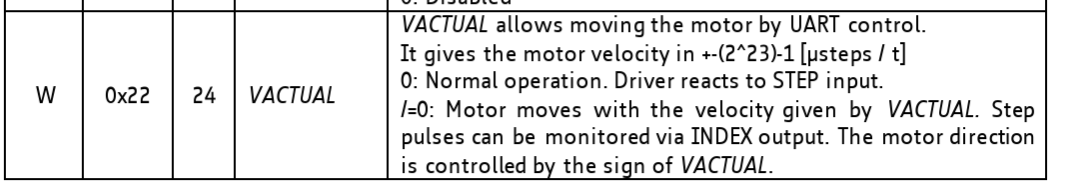
\includegraphics[width=0.9\textwidth]{assets/figures/tmc_vactual.png}
    \caption{Registre \texttt{V\_actual}}
    \label{fig:registre_vactual}
\end{figure}

Ce dernier permet donc de contrôler les moteurs directement par l'intermédiaire de l'interface UART, sans nécessiter la génération d'impulsions sur l'entrée \texttt{STEP}. La vitesse de rotation est déterminée par la valeur écrite dans le registre \texttt{V\_actual}, tandis que le sens de rotation est défini par le signe de cette valeur. Une valeur positive entraîne une rotation dans un sens, alors qu'une valeur négative provoque une rotation dans le sens inverse. Une valeur nulle arrête le moteur.

Cette méthode présente plusieurs avantages dans le cadre de ce projet. D'une part, elle réduit significativement la charge de calcul du microcontrôleur, qui n'a plus à générer des trains d'impulsions précis pour chaque moteur. D'autre part, elle simplifie l'architecture logicielle en permettant de piloter l'ensemble des paramètres du driver via une unique interface de communication.

Le contrôle des moteurs a donc été implémenté en utilisant ce registre plutôt que les entrées \texttt{STEP} et \texttt{DIR}.

La valeur à écrire dans le registre \texttt{V\_actual} est obtenue à partir de la vitesse angulaire de consigne selon les relations suivantes :

$$
f_{\mu step}=\frac{\omega}{2\pi}\times N_{step}\times N_{\mu}
$$

$$
V_{actual}=\frac{f_{\mu step}\times2^{24}}{f_{CLK}}
$$

En combinant les deux expressions, on obtient :

\begin{equation}
\begin{aligned}
V_{actual}=
\frac{\omega}{2\pi}
\times
N_{step}
\times
N_{\mu}
\times
\frac{2^{24}}{f_{CLK}}
\end{aligned}
\end{equation}

où :
\begin{itemize}
\item $\omega$ est la vitesse angulaire en \si{rad.s^{-1}} ;
\item $N_{step}$ est le nombre de pas par tour du moteur ;
\item $N_{\mu}$ est le nombre de micro-pas par pas ;
\item $f_{CLK}$ est la fréquence d'horloge du driver.
\end{itemize}

Les paramètres $N_{step}$, $N_{\mu}$ et $f_{CLK}$ sont définis dans le fichier \texttt{TMC2226.h}, ce qui permet d'adapter facilement la conversion à un autre moteur ou à une autre configuration de micro-pas.

Après des essais expérimentaux consistant à commander une vitesse de \SI{1}{tour.s^{-1}} pendant \SI{10}{s}, les moteurs réalisaient environ 9,75 tours avec la fréquence nominale de \SI{12}{MHz}. Afin d'obtenir une correspondance entre la vitesse commandée et la vitesse réelle, la fréquence d'horloge utilisée dans le calcul a été ajustée à \SI{11.7}{MHz}. Cette valeur est utilisée pour les deux drivers et permet d'obtenir une erreur de vitesse négligeable sur les essais réalisés.


\subsection{IMU}

L'\acrshort{imu}, un MPU6050 \cite{MPU6050_Datasheet}, est interfacé à l'aide de la bibliothèque Arduino \texttt{<Adafruit\_MPU6050.h>}. Cette bibliothèque fournit une interface de haut niveau permettant de communiquer facilement avec le capteur sans avoir à gérer directement les échanges sur le bus I\textsuperscript{2}C ni les registres internes du composant.

L'initialisation du capteur est réalisée par l'instanciation de la classe \texttt{Adafruit\_MPU6050}, suivie de l'appel à la méthode \texttt{begin()}. Cette dernière initialise automatiquement l'interface I\textsuperscript{2}C en utilisant la bibliothèque \texttt{Wire} d'Arduino, établit la communication avec le MPU6050 et vérifie la présence du capteur sur le bus. Aucune configuration supplémentaire de l'I\textsuperscript{2}C n'est donc nécessaire dans l'application.

Une fois la communication établie, plusieurs paramètres de fonctionnement du capteur sont configurés afin de l'adapter aux besoins du projet. Les réglages retenus sont les suivants :

\begin{itemize}
    \item \texttt{mpu.setAccelerometerRange(MPU6050\_RANGE\_2\_G)} : sélection d'une plage de mesure de $\pm2\,g$ pour l'accéléromètre. Cette configuration offre la meilleure résolution pour les faibles accélérations rencontrées lors du fonctionnement normal du robot.
    \item \texttt{mpu.setGyroRange(MPU6050\_RANGE\_500\_DEG)} : sélection d'une plage de mesure de $\pm500~^\circ/\mathrm{s}$ pour le gyroscope, permettant de mesurer les vitesses angulaires tout en conservant une bonne précision.
    \item \texttt{mpu.setFilterBandwidth(MPU6050\_BAND\_260\_HZ)} : configuration du filtre passe-bas numérique interne avec une bande passante de 260~Hz, offrant un compromis entre la réduction du bruit et la rapidité de réponse du capteur.
\end{itemize}

Les mesures fournies par le MPU6050 sont exprimées dans le repère du capteur. L'objectif est d'estimer l'angle d'inclinaison du robot autour de l'axe $X$, c'est-à-dire l'angle formé entre la normale au circuit imprimé (perpendiculaire à la carte électronique sur laquelle est monté le capteur) et la verticale.

Après l'acquisition des mesures de l'accéléromètre et du gyroscope à l'aide de la fonction \texttt{getEvent()}, une première estimation de l'angle est obtenue à partir de l'accéléromètre :

\begin{lstlisting}[language=C++, caption={Calcul de l'angle et filtre complémentaire}, label={lst:imu_complementary_filter}]
sensors_event_t accel, gyro, temp;
mpu.getEvent(&accel, &gyro, &temp);

// Accelerometer angle
float accelAngleX =
    atan2(accel.acceleration.x,
          sqrt(accel.acceleration.y * accel.acceleration.y +
               accel.acceleration.z * accel.acceleration.z)) *
    180.0f / PI;

// Gyro rate (Adafruit returns rad/s)
float gyroRateX = gyro.gyro.x * 180.0f / PI;

// Complementary filter
angleX = 0.9f * (angleX + gyroRateX * inner_loop_cnt)
       + 0.1f * accelAngleX;
\end{lstlisting}

Le calcul de \texttt{accelAngleX} repose sur le fait qu'en l'absence de déplacement latéral du robot, l'accéléromètre mesure principalement l'accélération de la pesanteur. Le vecteur gravité est alors projeté sur les trois axes du capteur. En considérant uniquement la rotation autour de l'axe $X$, l'angle d'inclinaison peut être déterminé grâce à la relation :

\begin{equation}
    \theta_X = \arctan\left(\frac{a_X}{\sqrt{a_Y^2+a_Z^2}}\right)
\end{equation}

où $a_X$, $a_Y$ et $a_Z$ représentent les accélérations mesurées selon les trois axes du MPU6050.

Le terme $\sqrt{a_Y^2+a_Z^2}$ correspond à la projection du vecteur gravité dans le plan $(Y,Z)$. La fonction \texttt{atan2()} est préférée à la fonction \texttt{atan()} car elle permet de déterminer correctement l'angle quel que soit le quadrant considéré et évite les divisions par zéro.

Lorsque le robot est parfaitement vertical, le vecteur gravité est principalement aligné avec l'axe $Z$ du capteur et l'angle calculé est proche de $0^\circ$. À mesure que le robot s'incline vers l'avant ou vers l'arrière, la composante de la gravité suivant l'axe $X$ augmente, ce qui fait varier l'angle estimé. Cette méthode fournit une mesure absolue de l'inclinaison, mais elle est sensible aux accélérations dues aux déplacements du robot ainsi qu'aux vibrations.

Le gyroscope fournit quant à lui la vitesse angulaire autour de l'axe $X$. La bibliothèque Adafruit retourne cette mesure en rad/s ; elle est donc convertie en degrés par seconde avant d'être intégrée au cours du temps selon la relation

\begin{equation}
    \theta_k = \theta_{k-1} + \omega \Delta t,
\end{equation}


où $\omega$ est la vitesse angulaire mesurée et $\Delta t$ correspond à la période d'échantillonnage (\texttt{inner\_loop\_cnt}). Cette estimation est très réactive mais présente une dérive progressive en raison des erreurs de mesure et du biais du gyroscope.

Afin de bénéficier des avantages de chacun des deux capteurs, un filtre complémentaire est utilisé. Celui-ci combine les deux estimations selon l'équation :


\begin{equation}
    \theta = 0.9\,(\theta_{\mathrm{gyro}}) + 0.1\,(\theta_{\mathrm{acc}})
\end{equation}


Le gyroscope assure ainsi la réactivité de la mesure sur les variations rapides, tandis que l'accéléromètre corrige progressivement la dérive à long terme. Ce filtre est largement utilisé pour les robots auto-équilibrés car il offre un excellent compromis entre précision, robustesse et coût de calcul, tout en étant suffisamment léger pour être exécuté à haute fréquence sur un microcontrôleur.

\subsection{Mesure de la batterie}

La mesure du niveau de tension de la batterie s'effectue en utilisant le ratio du pont diviseur (voir \ref{subsectin:pont_diviseur}). Ce ratio est inscrit dans le code sous forme de \texttt{define}, \texttt{D\_BATT\_RATIO}, et vaut $6.022$.

La tension de la batterie étant supérieure à la tension maximale admissible par l'entrée analogique du microcontrôleur, un pont diviseur résistif est utilisé afin d'abaisser la tension mesurée. L'entrée ADC mesure donc uniquement la tension présente aux bornes de la résistance inférieure du pont diviseur. Le rapport entre la tension réelle de la batterie et la tension mesurée par l'ADC est donné par le facteur \texttt{D\_BATT\_RATIO}.

La fonction \texttt{analogReadMilliVolts()} permet de récupérer directement la tension mesurée par l'ADC en millivolts après conversion. Cette valeur est ensuite multipliée par le ratio du pont diviseur afin de retrouver la tension réelle aux bornes de la batterie :
\begin{equation}
    V_{\mathrm{batterie}} = \frac{V_{\mathrm{ADC}} \times D_{\mathrm{BATT\_RATIO}}}{1000}
\end{equation}

où :
\begin{itemize}
    \item $V_{\mathrm{batterie}}$ correspond à la tension réelle de la batterie en volts ;
    \item $V_{\mathrm{ADC}}$ est la tension mesurée par le convertisseur analogique-numérique en millivolts ;
    \item $D_{\mathrm{BATT\_RATIO}}$ est le rapport de conversion du pont diviseur.
\end{itemize}

L'implémentation logicielle correspondante est présentée ci-dessous :

\begin{lstlisting}[language=C++, caption={Mesure de la tension batterie}, label={lst:battery_measurement}]
float read_battery()
{
  uint32_t voltage = analogReadMilliVolts(D_PIN_BATTERY_LVL);
  float battery_voltage = voltage * D_BATT_RATIO / 1000; // [V]
  return battery_voltage;
}
\end{lstlisting}

Ainsi, la valeur retournée par la fonction correspond directement à la tension d'alimentation de la batterie en volts, indépendamment de la division réalisée par le circuit de mesure. Cette information est ensuite utilisée afin de déterminer le niveau de charge de la batterie en pourcentage.

Afin d'estimer ce niveau de charge, deux tensions de référence sont définies dans le programme :

\begin{lstlisting}[language=C++]
#define D_BATT_MIN_V 14.70
#define D_BATT_MAX_V 16.00
\end{lstlisting}

La tension \texttt{D\_BATT\_MIN\_V} correspond au seuil considéré comme une batterie vide, tandis que \texttt{D\_BATT\_MAX\_V} représente la tension d'une batterie complètement chargée. Dans cette plage de fonctionnement, la tension mesurée est convertie en pourcentage à l'aide d'une fonction de mise à l'échelle linéaire (\textit{mapping}) :

\[
\mathrm{Niveau}_{\mathrm{batterie}} =
\frac{V_{\mathrm{batterie}}-V_{\mathrm{min}}}
{V_{\mathrm{max}}-V_{\mathrm{min}}}
\times 100
\]

où $V_{\mathrm{batterie}}$ est la tension mesurée, $V_{\mathrm{min}}$ la tension minimale définie par \texttt{D\_BATT\_MIN\_V} et $V_{\mathrm{max}}$ la tension maximale définie par \texttt{D\_BATT\_MAX\_V}.

La valeur obtenue est ensuite limitée entre $0$ et $100\,\%$ afin d'éviter des valeurs incohérentes lorsque la tension mesurée sort de la plage définie. Ainsi, une tension inférieure ou égale à $14.70\,V$ correspond à une batterie considérée comme vide, tandis qu'une tension supérieure ou égale à $16.00\,V$ correspond à une batterie pleine.
Cette approximation linéaire permet d'obtenir une indication simple et suffisamment précise de l'état de charge pour la supervision du système. Cependant, elle ne représente pas une estimation exacte de l'état de charge réel de la batterie. En effet, la courbe de décharge d'une batterie de type \acrshort{lipo} n'est pas linéaire : la tension reste relativement stable sur une grande partie de la décharge, puis chute rapidement lorsque la batterie approche de sa tension minimale. De plus, la tension mesurée dépend également de plusieurs paramètres tels que la température, le courant consommé par la charge et l'historique de charge de la batterie. Le pourcentage calculé doit donc être considéré comme une estimation permettant principalement de surveiller l'autonomie restante et de détecter une tension critique.

\section{Algorithmes de contrôle}


Cette partie décrit l'architecture logicielle utilisée pour contrôler le robot auto-équilibré. Le contrôle repose sur une structure en cascade composée de deux boucles de régulation.

La boucle externe est dédiée au contrôle de la vitesse du robot. Elle compare la vitesse mesurée avec la consigne utilisateur et génère une consigne d'inclinaison \texttt{theta\_target} permettant au robot d'accélérer ou de ralentir.

La boucle interne est dédiée au maintien de l'équilibre. Elle utilise la mesure d'inclinaison fournie par l'\acrshort{imu} afin de corriger rapidement la position du robot en agissant directement sur la vitesse des moteurs.

Le role de la boucle interne est de suivre la consigne imposée par la boucle externe.

Cette architecture permet de séparer deux dynamiques différentes : la dynamique lente du déplacement et la dynamique rapide de stabilisation. La boucle interne est exécutée à une fréquence élevée afin de compenser rapidement les perturbations, tandis que la boucle externe est exécutée plus lentement afin d'éviter des corrections trop brusques.   
\subsection{Structure du correcteur PID}

La structure utilisée est définie comme suit :

\begin{lstlisting}[language=C++, caption={Structure de données d'un contrôleur PID}, label={lst:pid_structure}]
typedef struct PIDController
{
  float kp;
  float ki;
  float kd;

  float integral;
  float previousError;

  float outputMin;
  float outputMax;
} PIDController;
\end{lstlisting}

Les trois premiers paramètres correspondent aux gains du correcteur :
\begin{itemize}
    \item \texttt{kp} est le gain proportionnel. Il définit la réaction immédiate du contrôleur face à une erreur ;
    \item \texttt{ki} est le gain intégral. Il permet de supprimer une erreur statique en accumulant l'erreur au cours du temps ;
    \item \texttt{kd} est le gain dérivé. Il permet d'anticiper les variations rapides de l'erreur en limitant les oscillations.
\end{itemize}

Les variables \texttt{integral} et \texttt{previousError} permettent de conserver l'état du correcteur entre deux appels successifs. En effet, contrairement au terme proportionnel qui ne dépend que de l'erreur actuelle, les termes intégral et dérivé nécessitent de connaître l'historique des mesures.

La fonction \texttt{PID\_update()} réalise le calcul de la commande à chaque itération de la boucle de contrôle. Le calcul du terme dérivé est effectué à partir de la variation de l'erreur :

\[
D = \frac{e(k)-e(k-1)}{\Delta t}
\]

où $e(k)$ représente l'erreur actuelle et $\Delta t$ la période d'échantillonnage.

Le terme intégral est calculé par accumulation :

\[
I(k)=I(k-1)+e(k)\Delta t
\]

La sortie du contrôleur est ensuite obtenue selon l'équation classique :

\[
u(k)=K_p e(k)+K_i I(k)+K_d D
\]

Une attention particulière est portée à la gestion de la saturation de la sortie. En effet, dans un système réel, la commande envoyée aux moteurs possède une limite physique. Lorsque cette limite est atteinte, l'intégration de l'erreur peut continuer à augmenter inutilement, provoquant un phénomène appelé \textit{windup}. Celui-ci entraîne généralement un dépassement important lorsque le système quitte la saturation.

Afin d'éviter ce comportement, une méthode d'\textit{anti-windup} est implémentée. L'intégrale n'est mise à jour que lorsque son évolution contribue à sortir de la saturation :

\begin{lstlisting}[language=C++]
if (!(saturatedHigh && error > 0) &&
    !(saturatedLow && error < 0))
{
    pid->integral += error * dt;
}
\end{lstlisting}

Ainsi, si la sortie du PID est déjà à sa valeur maximale et que l'erreur continue d'augmenter dans le même sens, l'intégrale est temporairement bloquée. Cette approche améliore la stabilité du système et réduit les temps de récupération après une saturation.

Enfin, la sortie du contrôleur est limitée entre \texttt{outputMin} et \texttt{outputMax} afin de respecter les contraintes physiques du système. Cette limitation est particulièrement importante pour la commande des moteurs, dont la vitesse maximale est définie par les caractéristiques mécaniques et électriques du robot.

\subsection{Calcul de la consigne d'inclinaison}

Afin de permettre au robot de se déplacer, il n'est pas suffisant de maintenir un angle nul. En effet, un robot auto-équilibré avance uniquement lorsqu'il s'incline légèrement dans la direction du mouvement souhaité. Cet angle d'inclinaison nécessaire est appelé \texttt{theta\_target} ou \textit{angle à atteindre}.

Lorsque le robot est parfaitement immobile, la consigne d'angle est proche de la verticale ($0^\circ$). Cependant, lorsqu'une vitesse de déplacement est demandée, le système doit créer une accélération horizontale afin de déplacer le centre de gravité. Pour générer cette accélération, le robot doit volontairement s'incliner légèrement.

Le calcul du \texttt{theta\_target} est réalisé par la boucle externe. La différence entre la vitesse cible et la vitesse mesurée est utilisée comme erreur d'entrée d'un premier correcteur PID :

\begin{lstlisting}[language=C++]
float speed_error = -(speed_target - speed);
theta_target = PID_update(&acceleration_PID,
                          speed_error,
                          outer_loop_cnt);
\end{lstlisting}

La sortie de ce correcteur correspond directement à l'angle souhaité $\theta_{target}$ transmis à la boucle interne. Si le robot est trop lent par rapport à la consigne, le contrôleur augmente l'angle demandé afin d'accélérer dans la direction souhaitée. Inversement, si la vitesse est trop élevée, l'angle demandé est réduit afin de ralentir le robot.

\subsection{Boucle de régulation d'équilibre}

La boucle de régulation d'équilibre une boucle rapide exécutée périodiquement. À chaque itération, l'angle du robot est mesuré à l'aide du MPU6050. L'estimation de l'angle est obtenue grâce au filtre complémentaire combinant l'accéléromètre et le gyroscope :

\begin{lstlisting}[language=C++]
angleX = 0.9f * (angleX + gyroRateX * inner_loop_cnt)
       + 0.1f * accelAngleX;
\end{lstlisting}

L'erreur d'inclinaison est ensuite calculée en prenant en compte :
\begin{itemize}
    \item l'angle d'équilibre du robot ;
    \item l'angle demandé par la boucle vitesse ;
    \item un offset de calibration du capteur ;
    \item l'angle réellement mesuré.
\end{itemize}

Le correcteur PID d'inclinaison génère alors une accélération permettant de ramener le robot vers son angle cible. Cette accélération est intégrée afin de calculer la nouvelle vitesse des moteurs.

La vitesse obtenue est ensuite limitée afin de protéger le système :

\begin{lstlisting}[language=C++]
motor_speed =
    motor_speed > D_MOTOR_MAX_SPEED ?
    D_MOTOR_MAX_SPEED :
    motor_speed < -D_MOTOR_MAX_SPEED ?
    -D_MOTOR_MAX_SPEED :
    motor_speed;
\end{lstlisting}

Enfin, la vitesse angulaire est convertie en vitesse de déplacement des moteurs pas à pas et envoyée aux drivers TMC2226 via UART :

\begin{lstlisting}[language=C++]
tmc2226_left.run_speed((int32_t)us_speed + motor_speed_delta);
tmc2226_right.run_speed(-(int32_t)us_speed + motor_speed_delta);
\end{lstlisting}

Le signe opposé appliqué aux deux moteurs permet de prendre en compte leur montage symétrique sur le robot.

La commande obtenue permet ainsi de stabiliser le robot autour de son angle d'équilibre tout en autorisant un déplacement contrôlé. La vitesse moteur résultante est ensuite combinée avec une éventuelle consigne de rotation avant d'être envoyée aux drivers moteurs.
\subsection{Contrôle de la rotation dans l'axe $Z$}

Afin de permettre au robot de tourner sur lui-même ou de suivre une trajectoire courbe, une différence de vitesse est appliquée entre les deux moteurs. Le principe utilisé est similaire à celui d'un véhicule à entraînement différentiel : lorsque les deux roues tournent à la même vitesse, le robot se déplace en ligne droite, tandis qu'une différence de vitesse entre les roues provoque une rotation autour de son centre.

Dans le cas d'un robot auto-équilibré à deux roues motrices, la vitesse de chaque moteur est obtenue en combinant la vitesse nécessaire au maintien de l'équilibre avec une composante de rotation :

$$
\omega_{gauche} = \omega_{équilibre} + \Delta\omega_{z}
$$

$$
\omega_{droite} = -\omega_{équilibre} + \Delta\omega_{z}
$$

Dans l'implémentation, cette composante de rotation correspond à la variable \texttt{motor\_speed\_delta} :

\begin{lstlisting}[language=C++]
float motor_speed_delta =
    rad_s_to_ustp_s(rotation_speed_target,
                    micro_stepping_value);

tmc2226_left.run_speed(
    (int32_t)us_speed + motor_speed_delta);

tmc2226_right.run_speed(
    -(int32_t)us_speed + motor_speed_delta);
\end{lstlisting}

La vitesse issue du correcteur d'équilibre (\texttt{us\_speed}) est appliquée avec un signe opposé aux deux moteurs afin de compenser leur montage mécanique inversé. Cette composante assure uniquement le déplacement avant ou arrière ainsi que la stabilisation du robot.

La variable \texttt{rotation\_speed\_target} est quant à elle une consigne indépendante permettant de commander la rotation. Elle est convertie en vitesse moteur par la fonction \texttt{rad\_s\_to\_ustp\_s()} afin d'être compatible avec les drivers TMC2226.

Ainsi :
\begin{itemize}
    \item lorsque \texttt{rotation\_speed\_target} vaut zéro, les deux moteurs compensent uniquement l'équilibre du robot et celui-ci avance en ligne droite ;
    \item lorsque \texttt{rotation\_speed\_target} est positive, une différence de vitesse est créée entre les roues, entraînant une rotation dans un sens ;
    \item lorsque \texttt{rotation\_speed\_target} est négative, la rotation s'effectue dans le sens opposé.
\end{itemize}

Cette méthode permet de découpler le contrôle de l'équilibre et celui de la direction. La boucle PID d'inclinaison reste ainsi uniquement responsable du maintien de la stabilité du robot, tandis que la commande de rotation modifie directement la vitesse relative des deux moteurs sans perturber la régulation d'équilibre.